\documentclass[a4paper,10pt]{scrartcl}
\usepackage[utf8]{inputenc}
\usepackage[italian]{babel}
\usepackage{hyperref}
\usepackage{graphicx}


\begin{document}

%opening
\title{BattleSheep}
\subtitle{Progetto di Sistemi Distribuiti}
\author{Giulio Biagini, Michele Corazza, Gianluca Iselli}

\maketitle

\begin{abstract}

\end{abstract}

\section{Introduzione}
Nell'ambito dei giochi multiplayer online è interessante osservare come sia 
possibile sfruttare paradigmi di comunicazione di tipo \textit{p2p} che non
prevedono, quindi, un server centrale che coordini la comunicazione fra client.
Tale approccio introduce certamente maggiori difficoltà implementative, ma
non esponendo un singolo point-of-failure risulta essere più tollerante ad
eventuali problemi di rete o sugli host.\newline
Il progetto qui descritto riguarda un'estensione multiplayer del famoso gioco
della \textit{Battaglia Navale} tradizionale, che sfrutti dunque il paradigma di
comunicazione p2p.\newline
La versione tradizionale del gioco prevede due giocatori che dapprima piazzano 
delle navi su una griglia bidimensionale di dimensioni prestabilite. Durante la 
partita vera e propria i due partecipanti si alternano dichiarando 
attacchi sulla griglia dell'avversario.\newline
Nella versione da noi implementata sono state apportate alcune modifiche.
Le navi sono state rimpiazzate da pecore sfruttando il 
gioco di parole fra battleship (battaglia navale) e battlesheep (battaglia fra
pecore). Al fine di semplificare le regole del gioco, poi, ciascuna pecora viene
piazzata singolarmente sulla griglia occupando, dunque, una sola cella, a
differenza delle navi che avrebbero occupato più spazio.\newline
L'estensione più importante riguarda però l'aspetto multigiocatore: ciascun 
partecipante dichiara, durante il suo turno, l'avversario da colpire e la 
cella obiettivo del suo attacco. Il risultato viene così comunicato a tutti i 
giocatori. Il vincitore del gioco è l'ultimo partecipante ad avere pecore vive 
sul proprio campo di battaglia. La classifica finale è data dall'ordine nel 
quale i giocatori perdono tutte le proprie pecore.


\section{Aspetti Progettuali}
Le principali componenti del software in esame sono due: un server di 
registrazione (lobby) e i client con i quali interagiscono i giocatori.
Il server di registrazione ha lo scopo di fornire un unico punto di accesso, 
in maniera da consentire ai client di conoscere le informazioni rilevanti degli 
altri peer. Una volta completato il suo compito, il server termina e tutte le 
comunicazioni successive avvengono con paradigma p2p fra i singoli client.
\\
Rispetto all'interazione con l'utente, i client forniscono la possibilità di 
specificare l'indirizzo IP su cui risiede il server della lobby, uno username 
che identifichi univocamente il giocatore e la posizione delle proprie pecore 
nel campo di gioco.
\\
Passiamo ora ad una trattazione più approfondita del protocollo di 
comunicazione da noi progettato.

\subsection{La comunicazione}


\section{Aspetti Implementativi}
Il software è stato implementato secondo il pattern architetturale \textbf{MVC},
anche noto come \textbf{Model-View-Controller}, il quale permette di creare una
architettura cosiddetta \textit{multi-tier}, ovvero nella quale le tre
componenti fondamentali di un programma sono suddivise in base ai compiti che
svolgono:
\begin{itemize}
	\item il \textit{modello}: che fornisce i metodi per accedere ai dati utili
	dell'applicazione;
	\item la \textit{vista}: la quale visualizza i dati del modello e si occpua
	dell'interazione con l'utente;
	\item il \textit{controller}: che riceve i comandi dall'utente e li attua
	modificando lo stato degli altri due componenti.
\end{itemize}
Nel nostro specifico caso, il modello si compone di tutte quelle classi atte a
mantenere i dati dell'applicazione. Abbiamo dunque l'oggetto che rappresenta il
campo di gioco dell'utente e degli avversari, l'oggetto che rappresenta i
giocatori impegnati nella partita, quello che astrae i dati degli host che si
registrano alla lobby con l'intenzione di partecipare al gioco,
eccetera\dots\newline
La vista è invece formata da tutta una serie di classi atte a permettere la
corretta visualizzazione dei dati, a partire dal frame per la registrazione fino
ad arrivare al frame di gioco.\newline
Vista la natura distribuita del programma, in questo specifico caso il
controller può essere pensato come a tutti quei meccanismi di interazione che
partono dall'utente ed hanno come obiettivo quello di modificare lo
\textit{stato globale} del gioco. Dunque, non soltanto le componenti software
che permettono di interagire direttamente con i dati mantenuti negli oggetti
del mio modello (locale), ma anche tutte le classi che permettono la
comunicazione fra gli host impegnati nella partita.\newline
Il software è stato realizzato in \textbf{Java}, un linguaggio orientato agli
oggetti, paradigma nel quale il modello MVC trova per sua stessa definizione un
impiego del tutto naturale.

\subsection{Modello}
Il modello\dots

\subsection{Vista}
Le classi della vista sono state implementate utilizzando la libreria
\textbf{Swing} fornita di default dal linguaggio.
\begin{figure}[!ht]
	\centering
	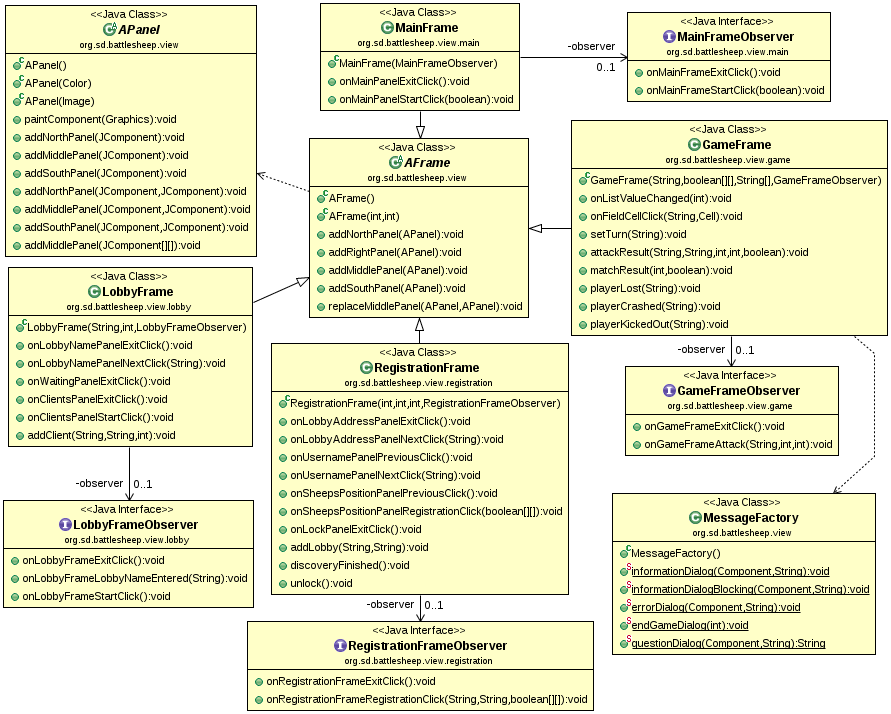
\includegraphics[scale=0.45,center]{core/imgs/UML/VistaBellaUML-noattr.png}
	\caption{Diagramma delle Classi - Vista}
	\label{figure:class_diagram_view}
\end{figure}
Come mostrato dal \textit{class diagram} in Figura \ref{figure:class_diagram_view} 
i 4 frame del gioco estendono un'unica
classe astratta appositamente creata per fornire una veste grafica di default:
l'\textit{AFrame}. Questo è essenzialmente un JFrame con un layout grafico
prestabilito che fornisce metodi utili per l'aggiunta e la sostituzione dei
pannelli che sono di volta in volta visualizzati. È qui che viene settato il
nome del programma come titolo della finestra, l'icona del gioco e la posizione sul display (al centro).\newline
Così come per i frame, tutti i pannelli estendono da un'unica classe,
l'\textit{APanel}. APanel fornisce anch'esso metodi per l'aggiunta dei vari oggetti che
lo popoleranno (label, aree di testo, bottoni, etc). Ogni frame mantiene al
proprio interno le istanze dei pannelli da mostrare.\newline
Un pattern molto importante e particolarmente sfruttato nell'implementazione
grafica di questo progetto è \textit{Observer}, il quale si basa su uno o più
oggetti (osservatori o observer) che vengono registrati e notificati
al verificarsi di determinate condizioni. Ogni pannello in grado di
generare eventi ha associata un'interfaccia che fornisce i metodi che
l'osservatore deve implementare per ricevere le notifiche. Dunque, ognuno dei 4
frame si comporta da osservatore nei confronti dei pannelli usati, implementando
le relative interfacce. Allo stesso modo i frame comunicano con le classi
sottostanti. Il dialogo con la vista avviene dunque in due modi:
\begin{itemize}
	\item quando dall'esterno si vuole comunicare con i frame, se ne usano i
	metodi che questi forniscono;
	\item quando invece la comunicazione parte dalla grafica, i frame usano i
	metodi forniti dalle rispettive interfacce che gli osservatori avranno il
	compito di implementare.
\end{itemize}



\subsubsection{Main Frame}
\begin{figure}[!h]
	\centering
	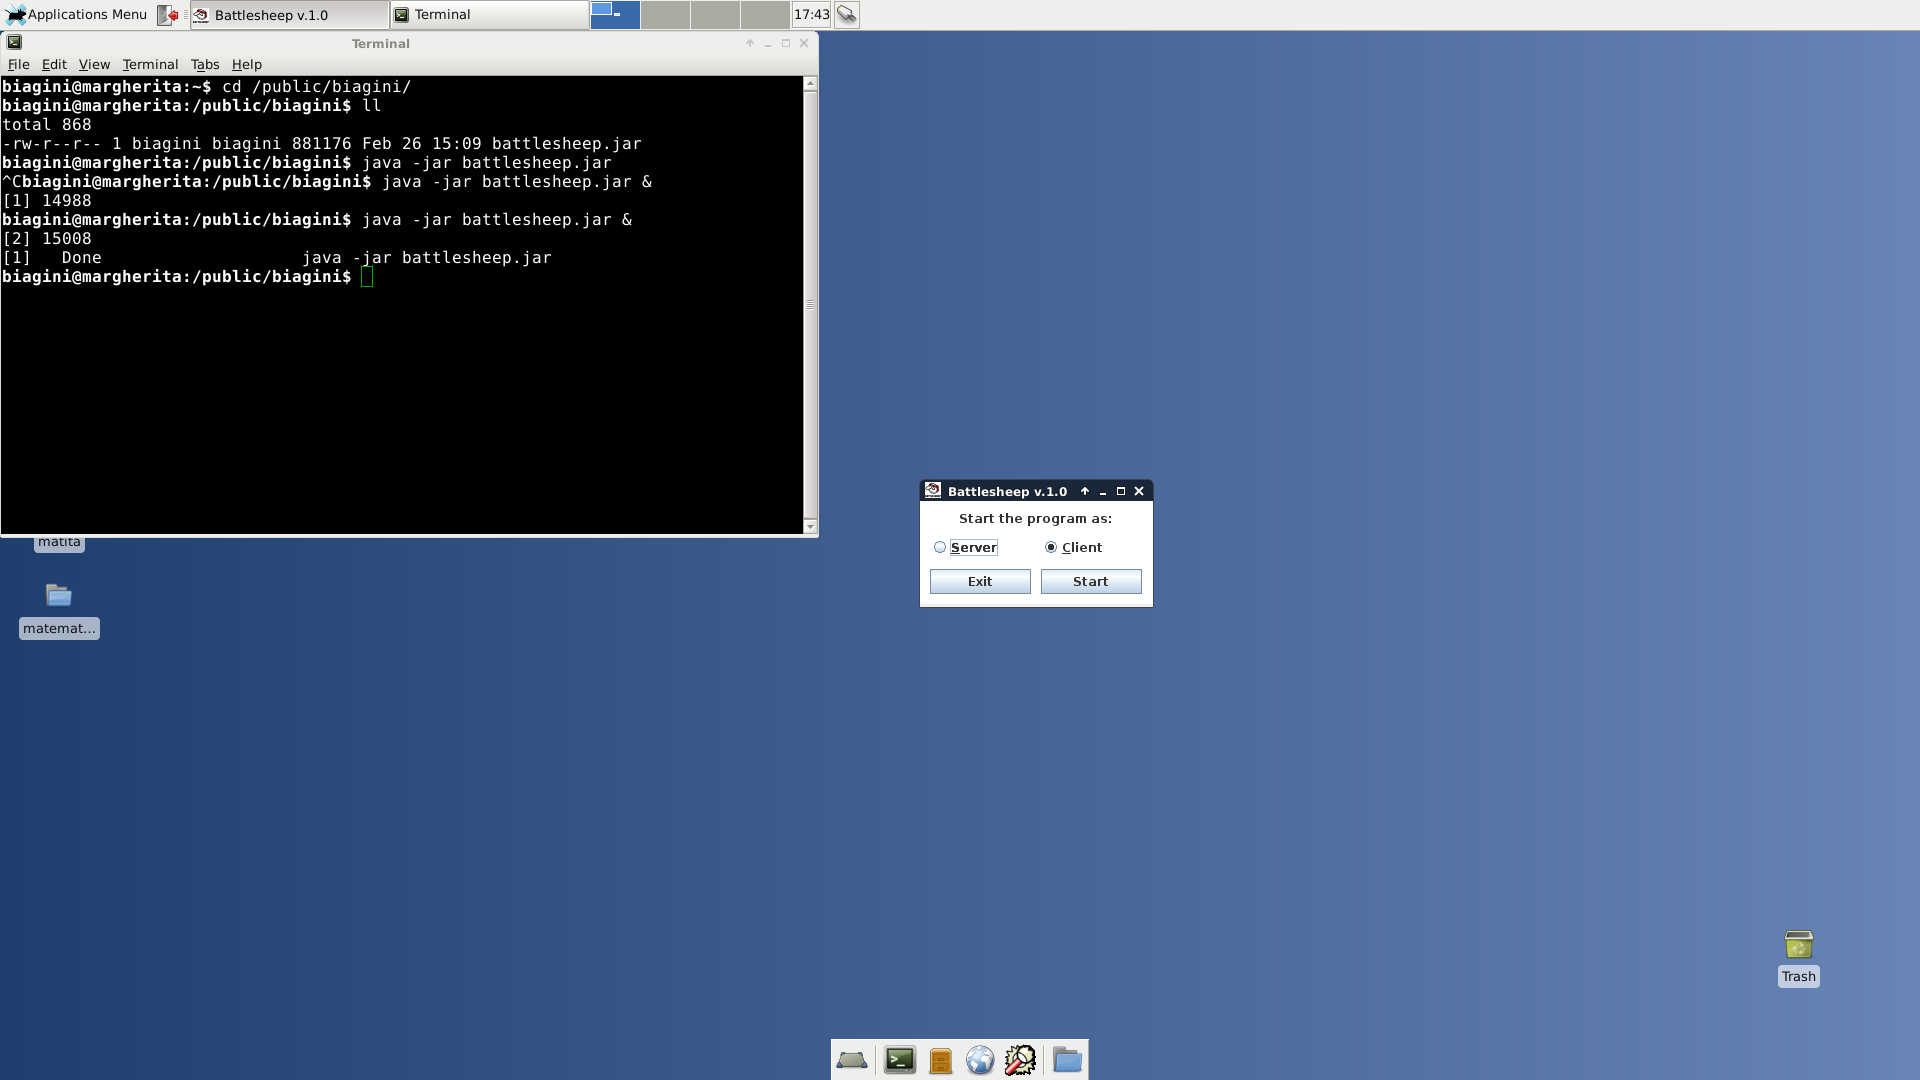
\includegraphics[scale=0.4]{core/imgs/gui/main_frame}
	\caption{Main Frame}
	\label{figure:main_frame}
\end{figure}
Il frame principale si compone di un unico pannello, il \textit{MainPanel} (Figura \ref{figure:main_frame}).
Così come detto in fase di progettazione,
questo frame ha il compito di
permettere all'utente la scelta della modalità nella quale avviare il programma:
se come server (lobby) o come client (game).\newline
Per la comunicazione verso l'esterno, il MainPanel ha un'interfaccia associata
che utilizza per notificare il MainFrame alla pressione dei bottoni ``Exit'' e
``Start'' il quale, a sua volta, tramite l'observer \textit{MainFrameObserver},
notifca il \textit{Main}.



\subsubsection{Lobby Frame}
\begin{figure}[!h]
	\begin{subfigure}{0.5\textwidth}
		\centering
		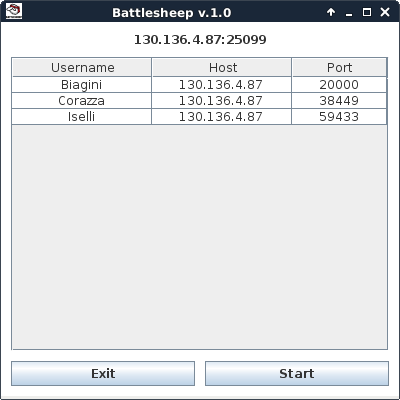
\includegraphics[scale=0.4]{core/imgs/gui/lobby_frame}
		\caption{Lobby Frame}
		\label{figure:lobby_frame}
	\end{subfigure}
	\begin{subfigure}{.5\textwidth}
		\centering
		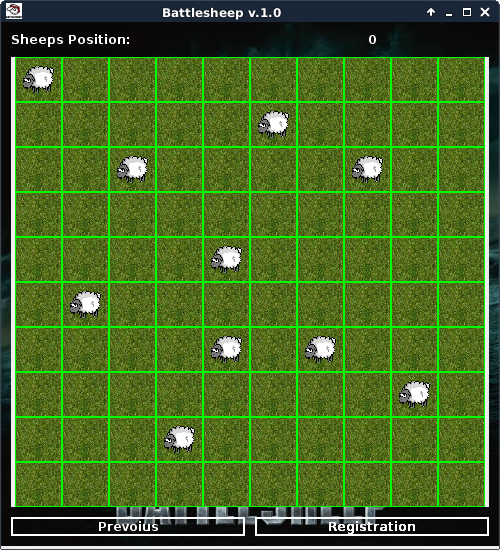
\includegraphics[scale=0.3]{core/imgs/gui/registration_frame}
		\caption{Registration Frame}
		\label{figure:registration_frame}
	\end{subfigure}
	\caption{}
\end{figure}
Il \textit{LobbyFrame} si compone di 3 pannelli, brevemente descritti in seguito. Il primo
pannello permette agli utenti di scegliere il nome della stanza. Ha due bottoni,
uno per l'uscita dal programma ed uno per l'avanzamento al pannello successivo.
Il secondo mostra una gif per l'attesa di connessioni da parte dei client ed ha
anch'esso un bottone di uscita. Il terzo ed ultimo pannello, visibile in Figura
\ref{figure:lobby_frame}, viene mostrato automaticamente non appena un client si
connette. Ospita due pulsanti: uno per l'uscita dal programma ed uno per l'avvio
della stanza.\newline
Quando uno dei bottoni di uscita viene premuto, il frame viene notificato dai pannelli.
Questo, a sua volta, propaga
l'informazione verso il proprio osservatore (\textit{Lobby}) tramite i metodi
forniti dall'interfaccia \textit{LobbyFrameObserver}. Lo stesso comportamento
viene attuato alla pressione del pulsante ``Start''. L'azione sul bottone
``Next'', invece, non viene propagata all'esterno ma serve al frame per sapere
quando visualizzare il secondo pannello.



\subsubsection{Registration Frame}
Il \textit{RegistrationFrame} si compone invece di 7 pannelli.\newline
Il comportamento di questo frame è del tutto simile a quello del LobbyFrame: gli
eventi scatenati dai pulsanti per l'avanzamento della registrazione (``Next'' e
``Previous'') sono usati internamente per la sostituzione dei vari pannelli,
mentre le azioni sui bottoni ``Exit'' e ``Registration'' sono propagate dal
frame verso il proprio osservatore (\textit{Battlesheep}) tramite l'interfaccia
\textit{RegistrationFrameObserver}.\newline
In Figura~\ref{figure:registration_frame} è mostrato il sesto pannello che
permette all'utente di scegliere la posizione delle proprie pecore nel campo di
gioco e di registrarsi alla lobby.



\subsubsection{Game Frame}
\begin{figure}[!h]
	\centering
	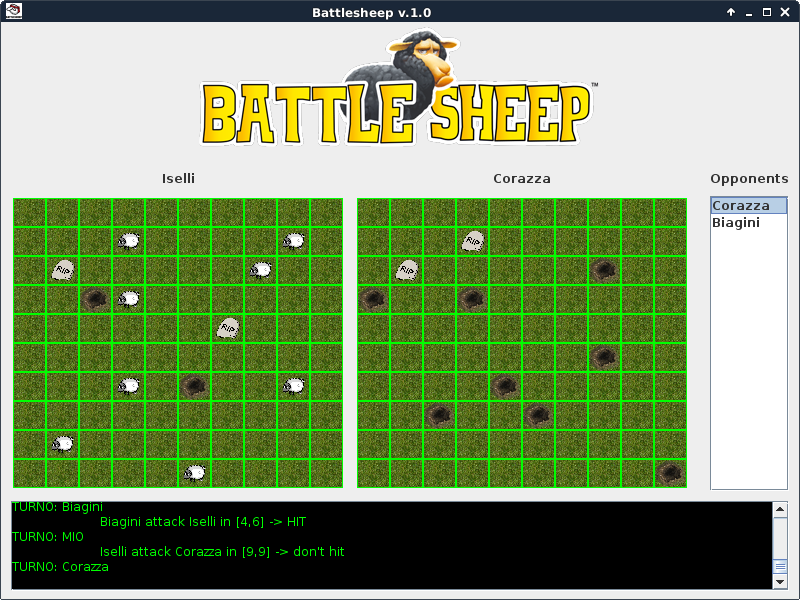
\includegraphics[scale=0.4]{core/imgs/gui/game_frame}
	\caption{Game Frame}
	\label{figure:game_frame}
\end{figure}
Il \textit{GameFrame}, mostrato in Figura~\ref{figure:game_frame}, è stato anch'esso
 implementato secondo le specifiche progettuali descritte in precedenza.\newline
La classe \textit{Battlesheep} comunica con questo frame tramite i metodi che
esso mette a disposizione, principalmente per informarlo di come è terminata la
partita per l'utente, per gli altri giocatori e su come si sono conclusi i vari
attacchi. Al contrario, il frame comunica con Battlesheep usando l'interfaccia
\textit{GameFrameObserver} per comunicare la volontà da parte dell'utente di
abbandonare il gioco o di attaccare un avversario in una daterminata posizione.

\subsection{Comunicazione}
La comunicazione\dots


\section{Valutazione e Conclusioni}
I test da noi effettuati hanno evidenziato la capacità del software di gestire 
guasti di tipo crash su uno qualsiasi dei client durante la comunicazione. Se 
la gestione di return parziali ha causato un leggero aumento della complessità 
del codice, tali errori non causano più inconsistenze durature, permettendo ai 
client di accordarsi autonomamente rispetto all'ordine delle mosse effettuate.
\\
L'implementazione della discovery delle lobby da parte dei client consente 
inoltre di fornire all'utente una semplice scelta delle stanze di gioco, senza 
assumere che essi conoscano a priori l'indirizzo IP. Naturalmente 
tale funzionalità è utile solo nel caso in cui i client si connettano ad un IP 
della propria sottorete, in quanto è impensabile fare discovery fra reti 
eterogenee senza prevedere un qualche server di appoggio esterno.
\\
Nonostante la semplicità del gioco scelto per il progetto, il protocollo di 
comunicazione implementato può essere facilmente generalizzabile a qualsiasi 
gioco a turni che proceda con una mossa per giocatore in un ordine prestabilito.
Sarebbe infatti sufficiente modificare le strutture dati relative alle mosse 
effettuate e cambiare leggermente le altre parti del codice per implementare un 
qualsiasi nuovo gioco a turni.
\\
Per aumentare la godibilità del gioco si potrebbe infine imporre al giocatore 
di inserire le pecore sul campo di gioco in celle contigue, in modo analogo a 
quanto avviene nella battaglia navale tradizionale. In questo modo ciascun 
attacco che ha avuto successo causerà una ricerca delle pecore rimanenti nelle celle adiacenti,
migliorando la gradevolezza complessiva del gioco.

\newpage

\section{Appendice}

\begin{figure}[!h]
	\centering
	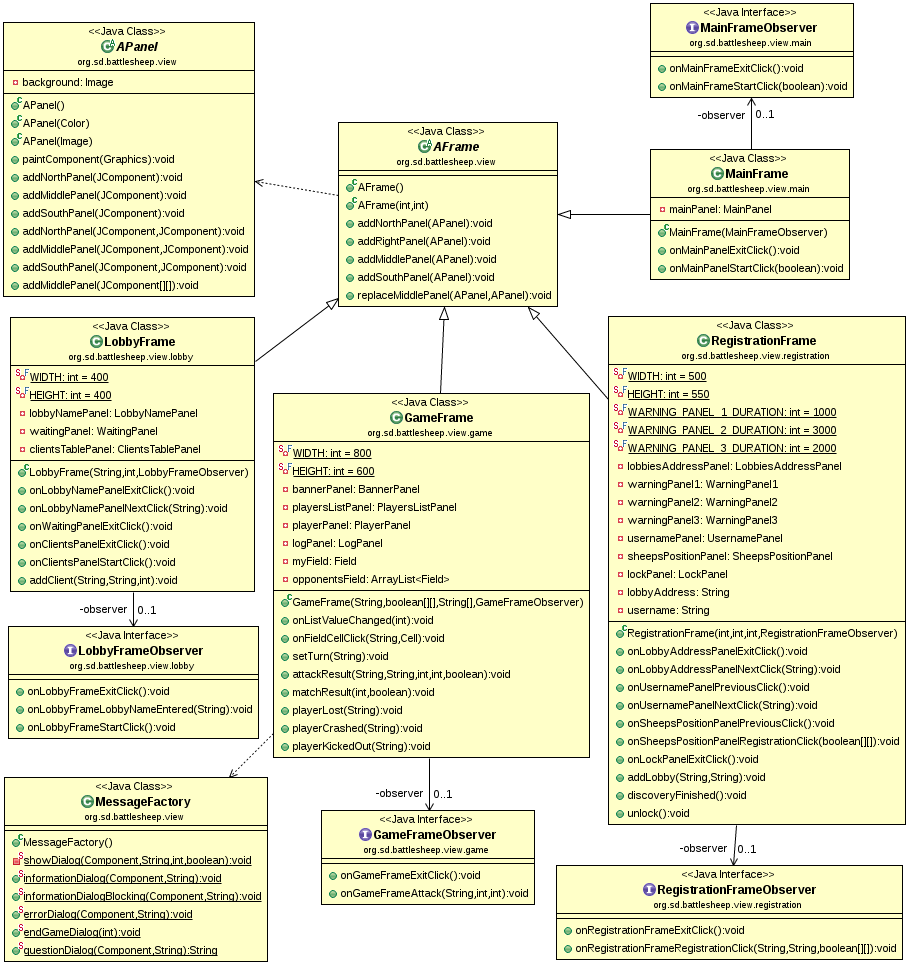
\includegraphics[scale=0.4]{core/imgs/UML/VistaBellaUML.png}
	\caption{Diagramma delle Classi - Vista}
	\label{figure:class_diagram_view}
\end{figure}


\begin{figure}[!ht]
    \centering
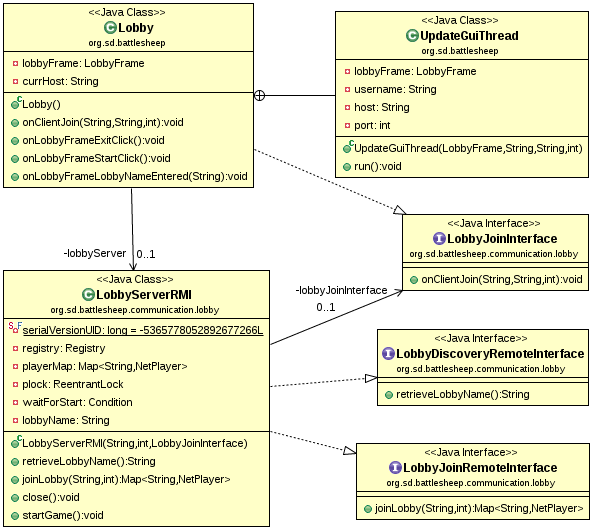
\includegraphics[width=1.0\textwidth]{core/imgs/UML/LobbyCommunicationUML.png}
    \caption{Diagramma delle classi, lobby server}
    \label{fig:classlobby}
\end{figure}

\begin{figure}[!ht]
    \centering
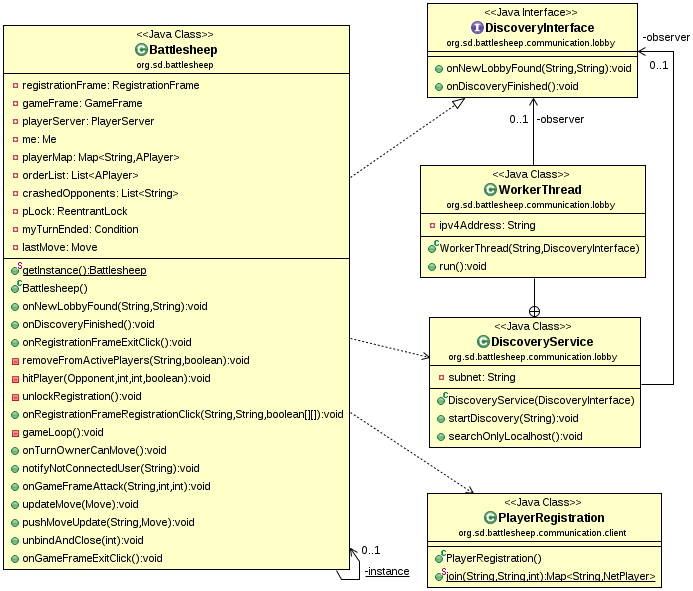
\includegraphics[width=1.0\textwidth]{core/imgs/UML/RegistrationBattlesheepCommunicationUML.png}
    \caption{Diagramma delle classi, discovery e registration lato client}
    \label{fig:classlobbyclientside}
\end{figure}

\begin{figure}[!ht]
    \centering
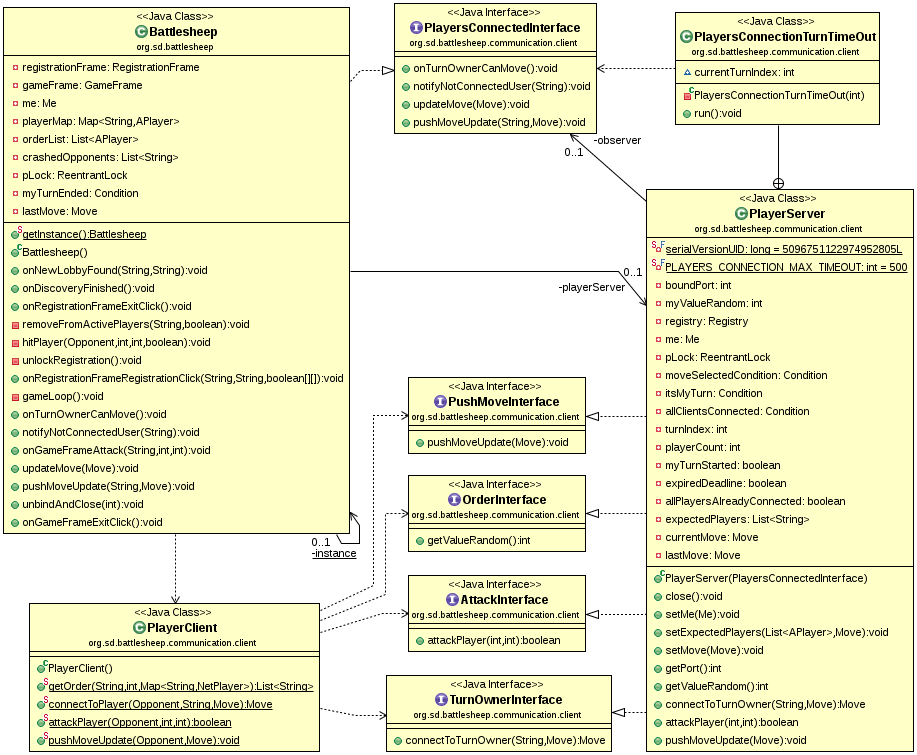
\includegraphics[width=1.0\textwidth]{core/imgs/UML/GameBattlesheepCommunicationUML.png}
    \caption{Diagramma delle classi, comunicazione fra client}
    \label{fig:classgame}
\end{figure}



\end{document}
